\documentclass[12pt]{article}

%%%%%%%%%%%%%%%%%%%%%%%%%%%%
%%%%%%%%%%%%%%%%%%%%%%%%%%%%
% Load in packages
\usepackage{amsmath}
\usepackage{float}
\usepackage{amssymb}
\usepackage{hyperref}
\usepackage{tikz}
\usepackage{pgfplots}
\pgfplotsset{compat=1.18} % or any recent version you use
\usepackage{graphicx}
\usepackage{enumitem}
\usepackage[top=1in, bottom=1in, left=1in, right=1in]{geometry}

%%%%%%%%%%%%%%%%%%%%%%%%%%%%
%%%%%%%%%%%%%%%%%%%%%%%%%%%%

\begin{document}

\begin{center}
\Large Chapter 15 Practice Problems

\medskip

\normalsize Elements of Microeconomics (discussion section 1)

\medskip

\small Rudy Kretschmar
\end{center}

\section*{Question 1}
Fill in the following table for a monopoly firm:
\begin{figure}[H]
    \centering
    \includegraphics[width=0.9\linewidth]{W12 chart1.png}
    \label{fig:placeholder}
\end{figure}
\vspace{4mm}
\textbf{Answer:}

\begin{figure}[H]
    \centering
    \includegraphics[width=0.9\linewidth]{W12 chart2.png}
    \label{fig:placeholder}
\end{figure}

\newpage

\section*{Question 2}
Assume that we have a monopoly firm in the market for internet. The market demand, average total cost, marginal cost for the firm, and marginal revenue for the firm is:
\[Q_D = 40 - 2P\]
\[ATC = \frac{50}{Q} + \frac{1}{4}Q\]
\[MC = \frac{1}{2}Q\]
\[MR = 20 - Q\]

\begin{enumerate}[label = (\alph*)]
    \item Graph these curves.
    \item Find the profit maximizing quantity for the firm ($Q^M$) and label it on your graph.
    \item What is the socially optimal quantity ($Q^E$)? Label it on your graph
    \item Calculate the profit for the firm and label it on your graph.
    \item Calculate the deadweight loss in this market and label it on your graph.
\end{enumerate}
\vspace{4mm}
\textbf{Answer:}
\begin{enumerate}[label = (\alph*)]
    \item Graph (green = $\pi$, red = $DWL$):
     \begin{center}
      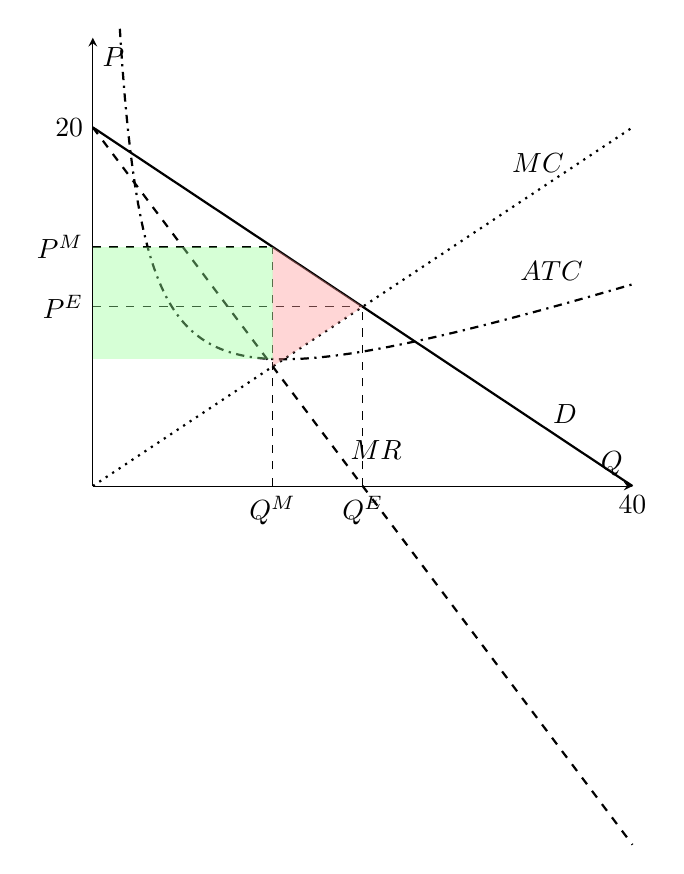
\begin{tikzpicture}
    \begin{axis}[
        axis lines = middle,
        xlabel = {$Q$},
        ylabel = {$P$},
        xmin = 0, xmax = 40,
        ymin = 0, ymax = 25,
        domain = 0:40,
        samples = 200,
        xtick=\empty,
        ytick=\empty,
        clip=false
    ]

        % Demand: Q = 40 - 2P => P = 20 - 0.5Q
        \addplot[thick] {20 - 0.5*x};
        \node at (axis cs: 35,4) {$D$};

        % MR: MR = 20 - Q => P = 20 - Q
        \addplot[thick, dashed] {20 - x};
        \node at (axis cs: 21,2) {$MR$};

        % MC: MC = 1/2 Q (so P = 1/2 Q)
        \addplot[thick, dotted] {.5*x};
        \node at (axis cs: 33,18) {$MC$};

        % ATC: ATC = 50/Q + (1/4)Q
        \addplot[thick, dashdotted, domain=2:40] {50/x + 0.25*x};
        \node at (axis cs: 34,12) {$ATC$};

        % Numeric values
        \def\QM{13.33}    % 40/3
        \def\PM{13.33}    % 40/3
        \def\QE{20}
        \def\PE{10}
        \def\ATCM{7.08}   % ATC(QM) ≈ 7.083
        \def\MCM{6.67}    % MC(QM) ≈ 6.667

        % Dashed guides for QM, PM
        \draw[dashed] (axis cs:\QM,0) -- (axis cs:\QM,\PM);
        \draw[dashed] (axis cs:0,\PM) -- (axis cs:\QM,\PM);

        % Dashed guides for QE, PE
        \draw[dashed] (axis cs:\QE,0) -- (axis cs:\QE,\PE);
        \draw[dashed] (axis cs:0,\PE) -- (axis cs:\QE,\PE);

        % Profit shading: between ATC(QM) and PM from 0 to QM
        \addplot[
            fill=green!40,
            draw=none,
            opacity=0.4
        ] coordinates {
            (0,\ATCM)
            (\QM,\ATCM)
            (\QM,\PM)
            (0,\PM)
        };

        % DWL shading: triangle between D and MC from QM to QE
        \addplot[
            fill=red!40,
            draw=none,
            opacity=0.4
        ] coordinates {
            (\QM,\MCM)   % MC at QM
            (\QM,\PM)    % D at QM (PM)
            (\QE,\PE)    % intersection of D and MC at QE
        };

        % ==== LABELS OUTSIDE THE AXES USING axis description cs ====
        % x-axis runs from Q = 0 to 40, so use fractions  Q/40
        % y-axis runs from P = 0 to 25, so use fractions  P/25

        % Q^M at x = QM/40 ≈ 0.333
        \node[below] at (axis description cs:0.333,0) {$Q^M$};

        % Q^E at x = 20/40 = 0.5
        \node[below] at (axis description cs:0.5,0) {$Q^E$};

        % P^M at y = PM/25 ≈ 0.533
        \node[left] at (axis description cs:0,0.533) {$P^M$};

        % P^E at y = 10/25 = 0.4
        \node[left] at (axis description cs:0,0.4) {$P^E$};

        % Intercepts:
        % Demand P-intercept at (0,20) => y = 20/25 = 0.8
        \node[left] at (axis description cs:0,0.8) {$20$};

        % Demand Q-intercept at (40,0) => x = 40/40 = 1
        \node[below] at (axis description cs:1,0) {$40$};

    \end{axis}
\end{tikzpicture} 
     \end{center}

     
    \item The firm maximizes profit where $MR = MC$:
    \begin{align*}
        MR &= MC \\
        20 - Q &= \frac{1}{2}Q \\
        20 & = \frac{3}{2}Q \\
        \frac{40}{3} & = Q^M
    \end{align*}

    \item The socially optimal quantity is the $Q$ where $MC = D$:
    First solve the demand curve for $P$:
    \begin{align*}
        Q_D & = 40 - 2P \\
        2P &= 40 - Q_D \\
        P &= 20 - \frac{1}{2}Q_D
    \end{align*}
    Then set the demand curve equal to marginal cost:
    \begin{align*}
        20 - \frac{1}{2} Q &= \frac{1}{2}Q \\
        20 = Q^E
    \end{align*} 

    \item The profit for a monopoly firm is the difference between the price they charge and their average total cost (at that $Q^M$) multiplied by the quantity sold. We know that the monopoly firms profit maximizing quantity is $Q^M = \frac{40}{3}$. So we can calculate the average total cost of the firm by plugging that value of $Q^M$ into the ATC function:
    \begin{align*}
        ATC(Q^M) &= \frac{50}{Q} + \frac{1}{4}Q \\
        ATC(Q^M) &= 50*\frac{3}{40} + \frac{40}{3}* \frac{1}{4} \\
        ATC(Q^M) &= \frac{15}{4} + \frac{40}{12} \\
        ATC(Q^M) &= \frac{85}{12}
    \end{align*}
    And we can calculate the monopoly firms price by plugging $Q^M$ into the demand equation:
    \begin{align*}
        Q_D &= 40 - 2P \\
        \frac{40}{3} & = 40 -2P \\
        2P &= \frac{120}{3} - \frac{40}{3} \\
        2P &= \frac{80}{3} \\
        P^* &= \frac{80}{6} = \frac{40}{3}
    \end{align*}
    Then the profit of the monopoly firm will be:
    \begin{align*}
        \pi &= (P^* - ATC) * Q^M \\
        \pi &= (\frac{40}{3} - \frac{85}{12})* \frac{40}{3} \\
        \pi &= (\frac{160 - 85}{12})*\frac{40}{3} \\
        \pi &= \frac{75}{12} * \frac{40}{3} \\
        \pi &= \frac{3000}{36} = \frac{250}{3}
    \end{align*}

    \item The deadweight loss in this market will be the firms price minus their marginal cost multiplied by the difference between the socially optimal quantity and the firms profit maximizing quantity, all times one half:
    \begin{align*}
        DWL &= \frac{1}{2}(P^* - MC) \times (Q^E - Q^M) \\
        &= \frac{1}{2}*(\frac{40}{3} - \frac{40}{6}) * (20 - \frac{40}{3}) \\
        &= \frac{1}{2}*\frac{20}{3} * \frac{20}{3} \\
        DWL &= \frac{1}{2}*\frac{400}{9} = \frac{400}{18} = \frac{200}{9}
    \end{align*}
\end{enumerate}

\section*{Question 3}
 Give a real world example of price discrimination, and explain how it increases social welfare.
\vspace{4mm}
 \textbf{Answer:}

\begin{enumerate}
    \item Movie theaters often charge lower ticket prices for students and seniors. 
Because these groups have more elastic demand, discounted prices allow the 
firm to serve consumers who would not purchase at the regular price, increasing 
total surplus and improving allocative efficiency.
    \item Airlines use price discrimination by charging business travelers higher fares 
than leisure travelers. By separating consumers by willingness to pay, airlines 
fill more seats that would otherwise go empty, increasing total surplus and 
reducing deadweight loss.
    \item Pharmaceutical companies sell the same drug at lower prices in low-income 
countries and higher prices in high-income countries. This expands access for 
price-sensitive consumers while still covering fixed R\&D costs, raising overall 
social welfare.
\end{enumerate}



\end{document}
